\documentclass[12pt, twoside]{article}
\usepackage[letterpaper, margin=1in, headsep=0.5in]{geometry}
\usepackage[english]{babel}
\usepackage[utf8]{inputenc}
\usepackage{amsmath}
\usepackage{amsfonts}
\usepackage{amssymb}
\usepackage{tikz}
%\usetikzlibrary{quotes, angles}

\usepackage{graphicx}
\usepackage{enumitem}
\usepackage{multicol}

\usepackage{fancyhdr}
\pagestyle{fancy}
\fancyhf{}
\renewcommand{\headrulewidth}{0pt} % disable the underline of the header

\fancyhead[LE]{\thepage}
\fancyhead[RO]{\thepage \\ Name: \hspace{4cm} \,\\}
\fancyhead[LO]{BECA / Dr. Huson / Geometry\\* Unit 7: Similarity\\* 8 January 2020}

\begin{document}
\subsubsection*{7.5 Do Now: Similarity transformations and the tangent function}
  \begin{enumerate}
  \item The diagram below shows $\triangle ABC$, with $\overline{AEB}$, $\overline{ADC}$, and $\angle ACB \cong \angle AED$. $AB=14$, $AD=8$, and $DE=4$.
  \begin{multicols}{2}
    \begin{enumerate}
        \item $\overline{AE} \rightarrow$ \rule{2cm}{0.15mm} \vspace{0.5cm}
        \item $\overline{AD} \rightarrow$ \rule{2cm}{0.15mm} \vspace{0.5cm}
        \item $\triangle ADE \sim$ \rule{2cm}{0.15mm} \vspace{0.5cm}
        \item What is the scale factor?\\[0.5cm] $k=$  \rule{2cm}{0.15mm}
        \item What is the length of $\overline{BC}$?
      \end{enumerate}
      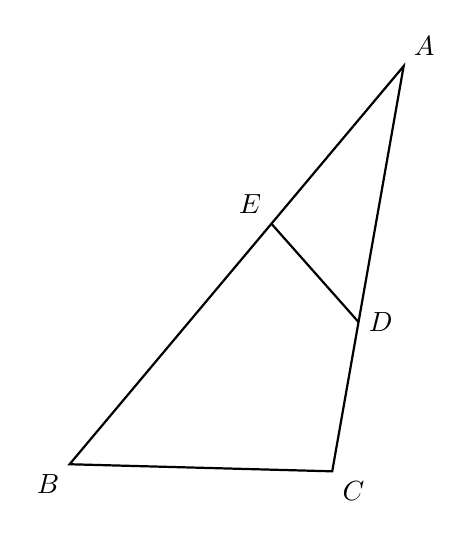
\begin{tikzpicture}[scale=1.1]
        \draw [thick]
        (0,0) node[above right] {$A$}--
        (230:6) node[below left] {$B$}--
        (260:4.75) node[below right] {$C$}--cycle;
        \draw [thick]
        (230:2.375) node[above left] {$E$}--
        (260:3) node[right] {$D$}--cycle;
      \end{tikzpicture}
    \end{multicols} \vspace{1.5cm}
 
   \item Given $\triangle JKL \sim \triangle MNO$. $m\angle J = 43^\circ$ and $m\angle L = 92^\circ$.\\[0.25cm]
   Find the measure of $\angle O$. \vspace{1.cm}

   \item Determine and state the transformation or sequence of transformations  applied to $\triangle ABC$, mapping it onto $\triangle PQR$, as shown.
   \begin{flushright}
       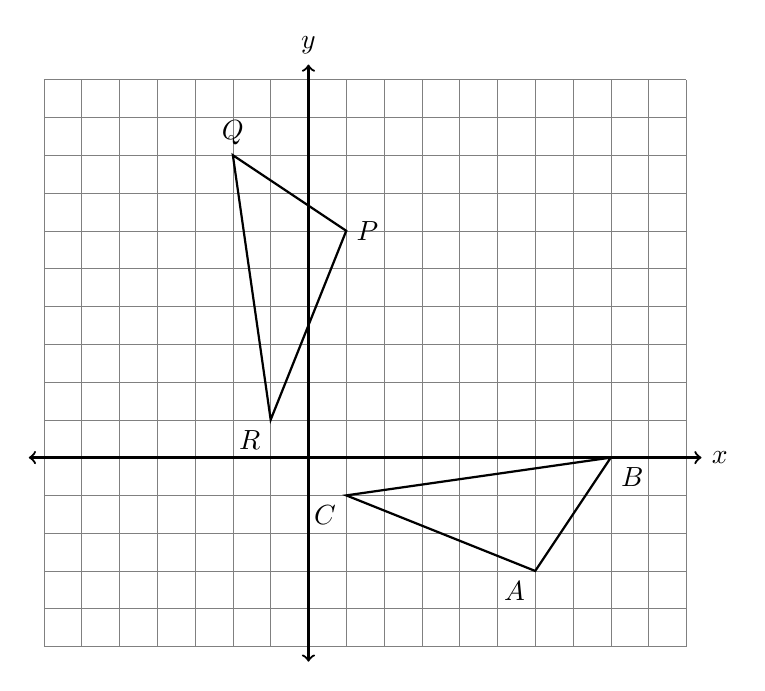
\begin{tikzpicture}[scale=.48]
         \draw [help lines] (-7,-5) grid (10,10);
         \draw [thick, <->] (-7.4,0) -- (10.4,0) node [right] {$x$};
         \draw [thick, <->] (0,-5.4)--(0,10.4) node [above] {$y$};

         \draw [thick]
         (6,-3) node[below left] {$A$}--
         (8,0) node[below right] {$B$}--
         (1,-1) node[below left] {$C$}--cycle;

         \draw [thick]
         (1,6) node[right] {$P$}--
         (-2,8) node[above] {$Q$}--
         (-1,1) node[below left] {$R$}--cycle;
       \end{tikzpicture}
     \end{flushright}
     
\newpage
  \item What series of transformations map $\triangle ABC$ onto $\triangle DEF$, shown below? Fully specify the transformations.
    \begin{flushright}
      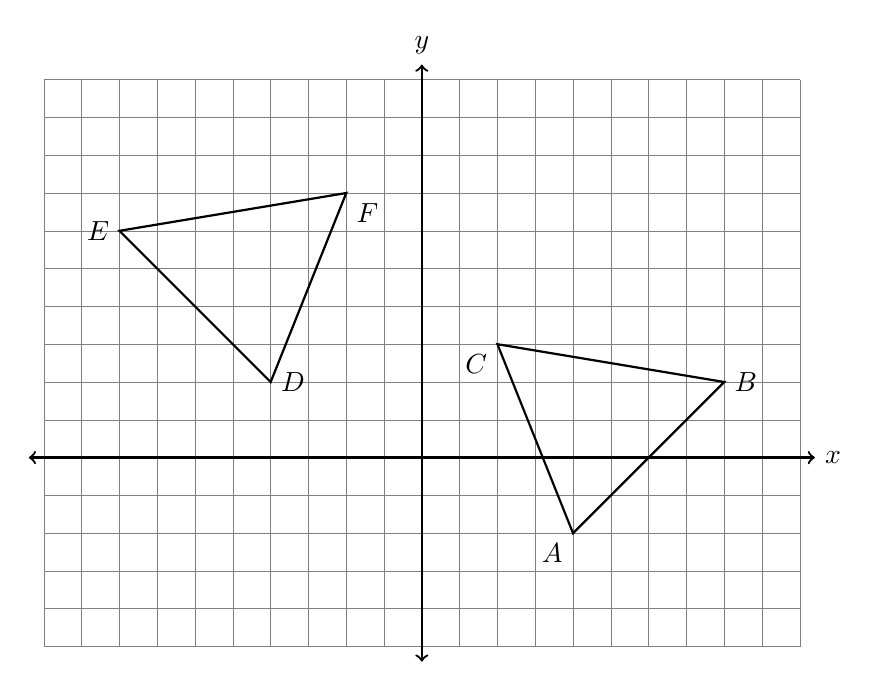
\begin{tikzpicture}[scale=.48]
        \draw [help lines] (-10,-5) grid (10,10);
        \draw [thick, <->] (-10.4,0) -- (10.4,0) node [right] {$x$};
        \draw [thick, <->] (0,-5.4)--(0,10.4) node [above] {$y$};
        \draw [thick]
          (4,-2) node[below left] {$A$}--
          (8,2) node[right] {$B$}--
          (2,3) node[below left] {$C$}--cycle;
        \draw [thick]
          (-4,2) node[right] {$D$}--
          (-8,6) node[left] {$E$}--
          (-2,7) node[below right] {$F$}--cycle;
      \end{tikzpicture}
    \end{flushright}

  \item The $\triangle ABC$ is reflected across $l$ to yield $\triangle A'B'C'$. $AB=3x+4$, $A'B'=5x-10$, and $BC=4x+12$. Find the length $B'C'$. %\vspace{2cm}
    \begin{flushright}
    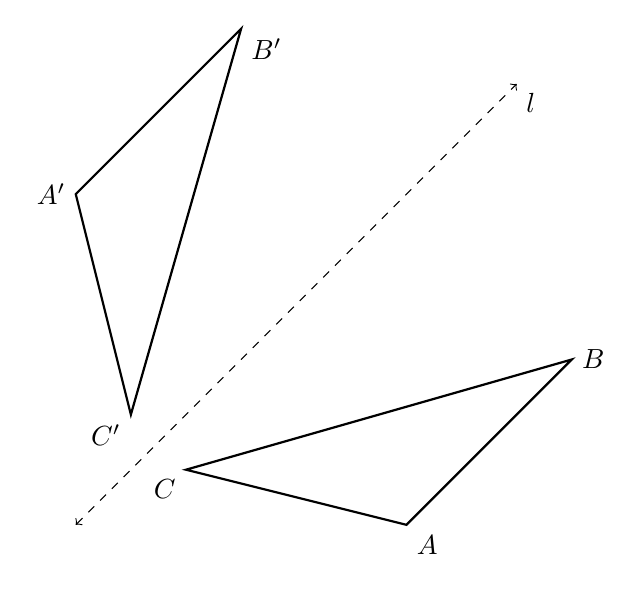
\begin{tikzpicture}[scale=.7]
      \draw [dashed, <->] (-1,-1)--(7,7) node[below right]{$l$};
      \draw [thick]
      (5,-1) node[below right] {$A$}--
      (8,2) node[right] {$B$}--
      (1,0) node[below left] {$C$}--cycle;
      \draw [thick]
      (-1,5) node[left] {$A'$}--
      (2,8) node[below right] {$B'$}--
      (0,1) node[below left] {$C'$}--cycle;
    \end{tikzpicture}
  \end{flushright}



\newpage  
\subsubsection*{Modeling: Mark each diagram and write and equation. Do Not Solve!}
  \item Given right $\triangle JKL$ with $\overline{JK} \perp \overline{KL}$, $JK=11$, $m\angle J=18^\circ$. Let $x$ be the length of the side opposite $\angle J$, $x=KL$.\\[0.5cm] 
  Write an equation expressing $\tan \angle J$ as a ratio of \emph{opposite} over \emph{adjacent}. \hfill (2 stars)
      \begin{flushright}
          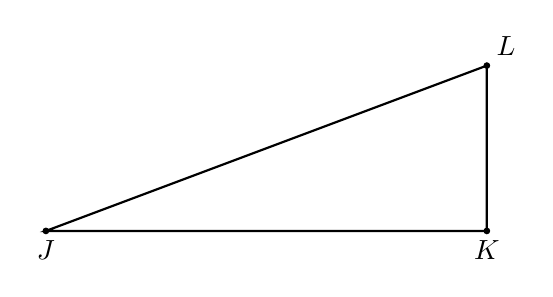
\begin{tikzpicture}[scale=0.7]
            \draw [thick](-1,0)--(7,0)--(7,3)--cycle;
            \draw [fill] (-1,0) circle [radius=0.05] node[below]{$J$};
            \draw [fill] (7,0) circle [radius=0.05] node[below]{$K$};
            \draw [fill] (7,3) circle [radius=0.05] node[above right]{$L$};
          \end{tikzpicture}
        \end{flushright}

  \item Given right $\triangle ABC$ with $m\angle C =90^\circ$, $BC=5$, $m\angle A=38^\circ$. Let $x=AC$. \hfill (2 stars)
    \begin{flushright}
        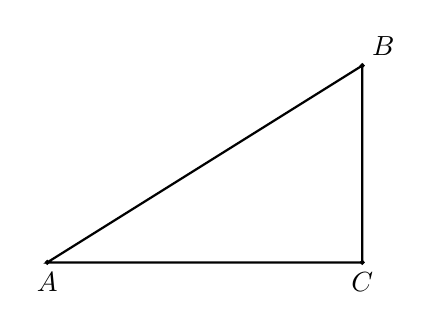
\begin{tikzpicture}[scale=0.5]
          \draw [thick](-1,0)--(7,0)--(7,5)--cycle;
          \draw [fill] (-1,0) circle [radius=0.05] node[below]{$A$};
          \draw [fill] (7,0) circle [radius=0.05] node[below]{$C$};
          \draw [fill] (7,5) circle [radius=0.05] node[above right]{$B$};
        \end{tikzpicture}
      \end{flushright}

  \item Given right $\triangle ABC$ with $m\angle C =90^\circ$, $BC=6$, $AC=22$, and $m\angle A=x^\circ$. \hfill (2 stars)
  \begin{flushright}
    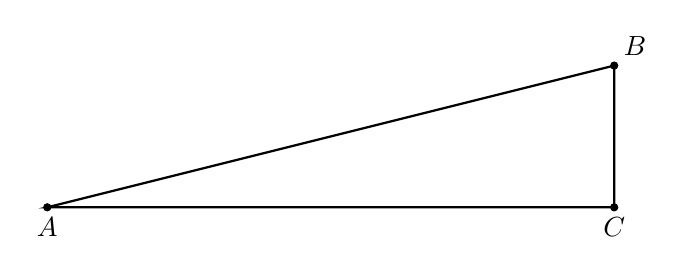
\begin{tikzpicture}[scale=0.9]
      \draw [thick](-1,0)--(7,0)--(7,2)--cycle;
      \draw [fill] (-1,0) circle [radius=0.05] node[below]{$A$};
      \draw [fill] (7,0) circle [radius=0.05] node[below]{$C$};
      \draw [fill] (7,2) circle [radius=0.05] node[above right]{$B$};
    \end{tikzpicture}
  \end{flushright}
  
  \item Given right $\triangle ABC$ with $\overline{AC} \perp \overline{BC}$, $BC=7$, $m\angle B=55^\circ$. Let $x=AC$. \hfill (3 stars)
  \begin{flushright}
    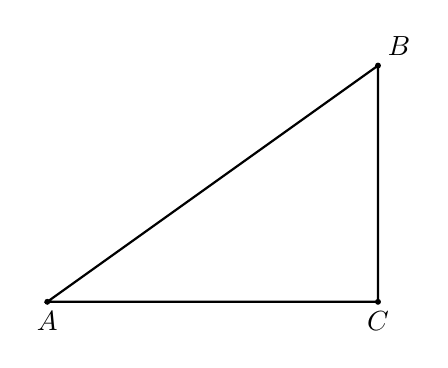
\begin{tikzpicture}[scale=0.6]
      \draw [thick](-1,0)--(6,0)--(6,5)--cycle;
      \draw [fill] (-1,0) circle [radius=0.05] node[below]{$A$};
      \draw [fill] (6,0) circle [radius=0.05] node[below]{$C$};
      \draw [fill] (6,5) circle [radius=0.05] node[above right]{$B$};
    \end{tikzpicture}
  \end{flushright}

\newpage
\subsubsection*{Mastery topic: Algebraic solution}
\item Solve each equation for $x$, rounding to the nearest hundredth.
  \begin{multicols}{2}
  \begin{enumerate}
  \item $\displaystyle \tan 75^\circ = \frac{x}{15}$ \vspace{5cm}
  \item $\displaystyle \tan 26^\circ = \frac{4}{x}$
  \item $\displaystyle \sin 46^\circ  = \frac{x}{3.5}$ \vspace{5cm}
  \item $\displaystyle \cos 35^\circ = \frac{x}{10}$
  \end{enumerate}
  \end{multicols}
  \vspace{6cm}

\item Solve for $x$, rounding to the nearest whole degree.
  \begin{multicols}{2}
  \begin{enumerate}
  \item $\displaystyle x = \tan^{-1} (\frac{2}{3.5})$ \vspace{4cm}
  \item $\displaystyle \tan x^\circ = \frac{17}{9}$ \vspace{4cm}
  \end{enumerate}
  \end{multicols}

\end{enumerate}
\end{document}